\XeTeXlinebreaklocale "zh"
\XeTeXlinebreakskip = 0pt plus 1pt

\documentclass[11pt,a4paper]{article}

\usepackage{xltxtra,fontspec,xunicode}
\usepackage{amsthm, amsmath, amssymb, amsfonts}
\usepackage{abstract}
\usepackage{subcaption}
\usepackage{graphicx,float} 
\usepackage{minted}

\defaultfontfeatures{Mapping=tex-text,Scale=MatchLowercase}
\setmainfont{DejaVu Serif}
\setsansfont{DejaVu Sans}
\setmonofont{DejaVu Sans Mono}
\usepackage[slantfont,boldfont]{xeCJK} % 允许斜体和粗体
\setCJKmainfont{WenQuanYi Zen Hei}
\setCJKsansfont{WenQuanYi Zen Hei}
\setCJKmonofont{WenQuanYi Zen Hei Mono}

\usepackage{titling}

\renewcommand\refname{参考文献} 

\title{人物信息检索系统的功能及其实现}
\author{周聿浩\\ \small{2016011347}}

\begin{document}
\maketitle
\section{简介}
这是一个利用Django搭建的一个人物信息检索系统,大约从Wikipedia爬取了10000个人物信息,并且提取了其中Infobox的对应信息。

\begin{figure}[H]
	\centering
	\begin{subfigure}{.49\textwidth}
		\centering
		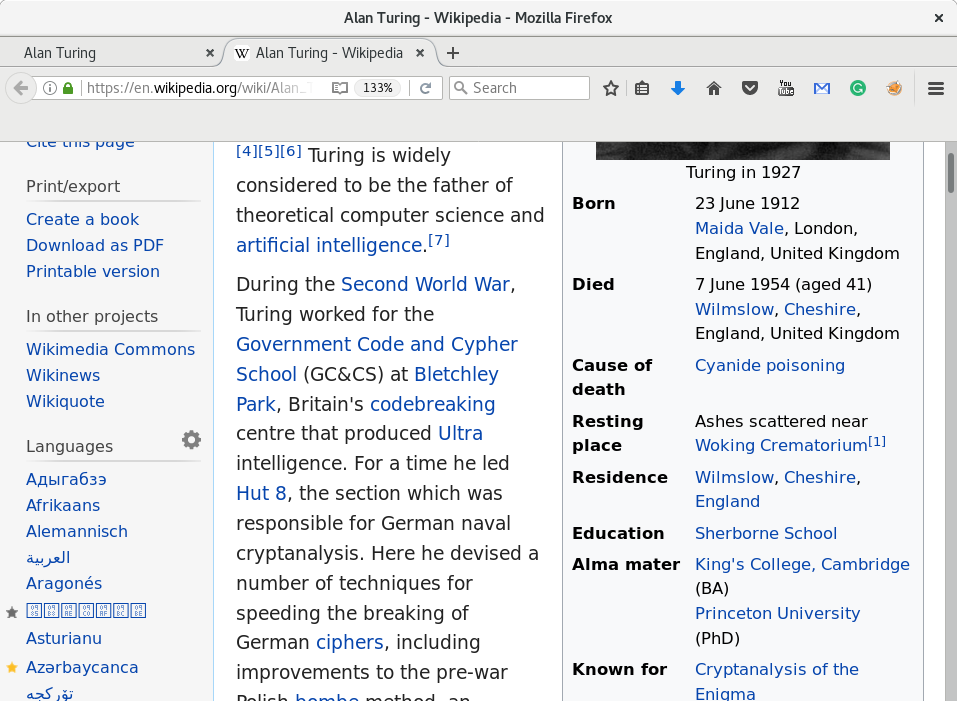
\includegraphics[width=\linewidth]{wiki.png}
	\end{subfigure}
	\hfill
	\begin{subfigure}{.49\textwidth}
		\centering
		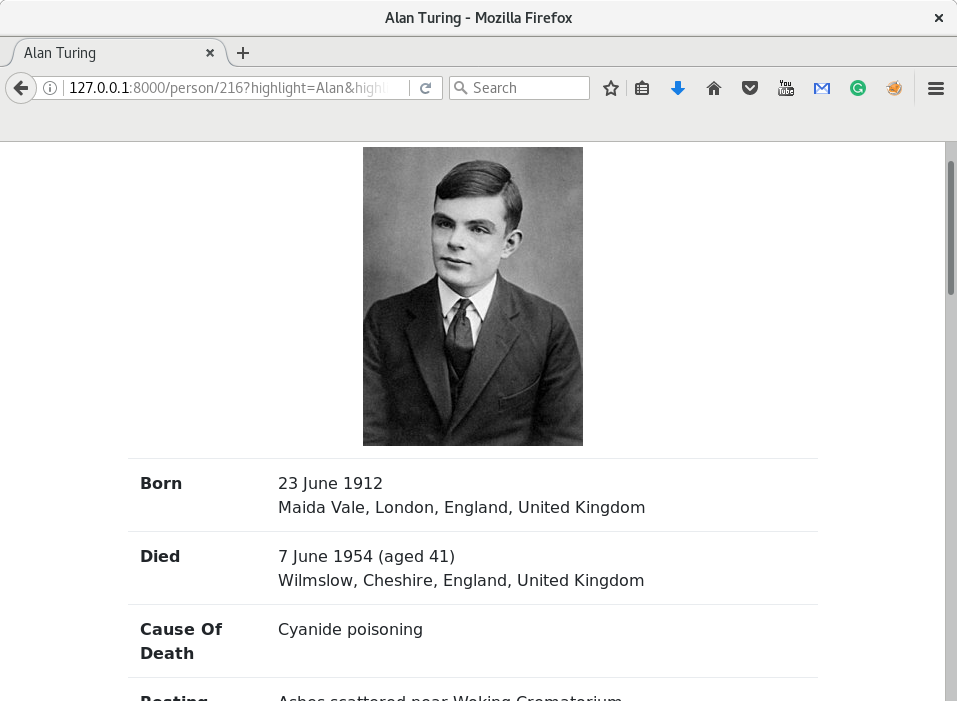
\includegraphics[width=\linewidth]{turing-1.png}
	\end{subfigure}
	\caption{对于Wikipedia中爬取的信息,我们重新组织了其格式并且进行显示。}
\end{figure}

\begin{figure}[H]
	\centering
	\begin{subfigure}{.49\textwidth}
		\centering
		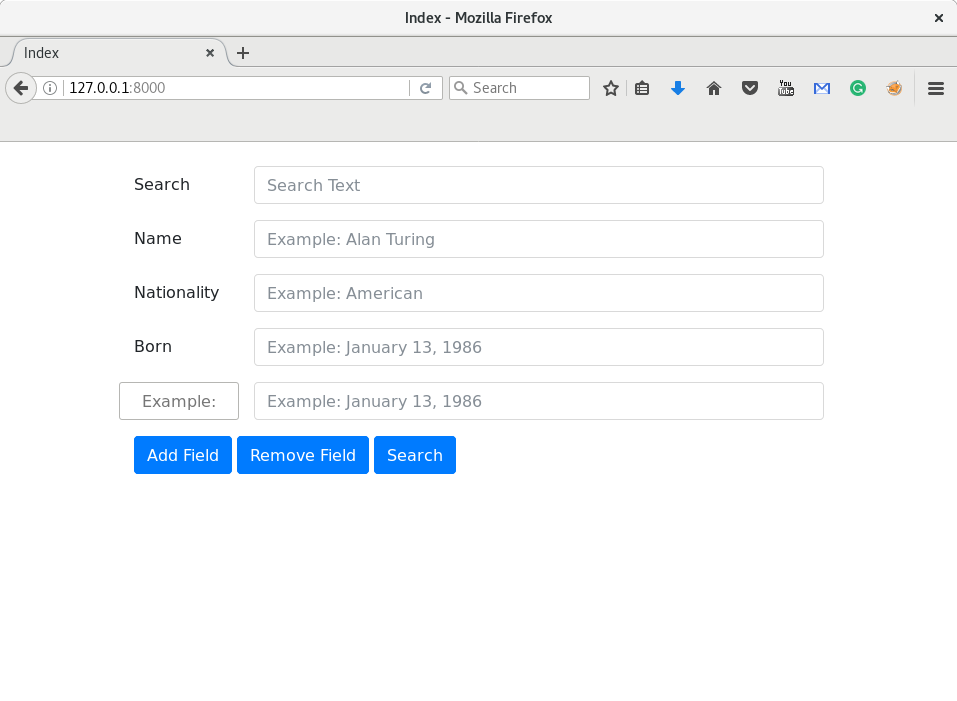
\includegraphics[width=\linewidth]{img-1.png}
	\end{subfigure}
	\hfill
	\begin{subfigure}{.49\textwidth}
		\centering
		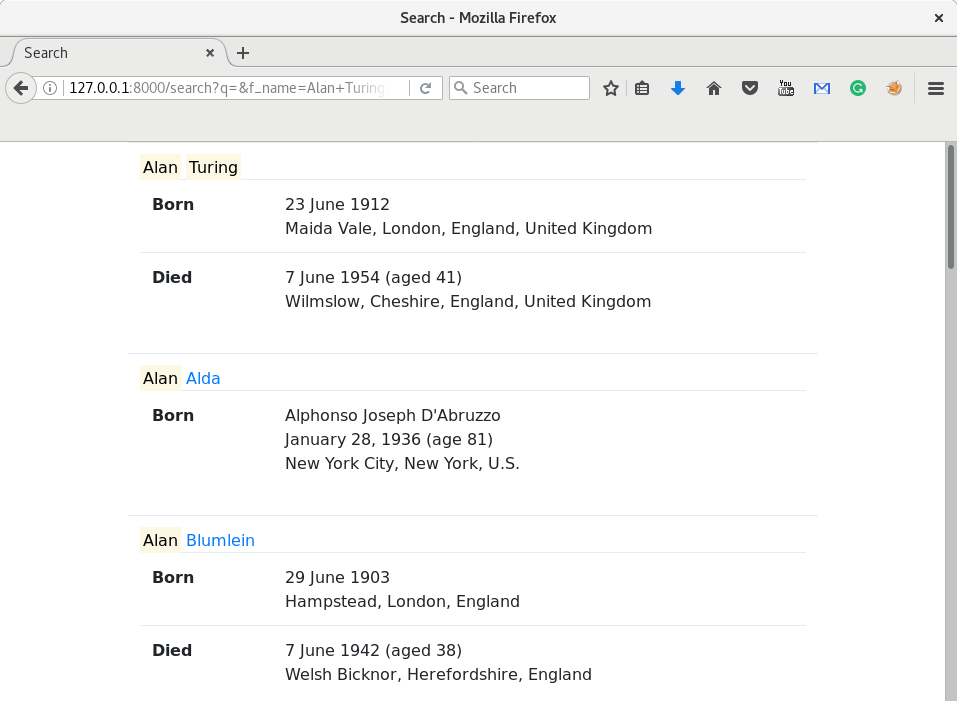
\includegraphics[width=\linewidth]{img-2.png}
	\end{subfigure}
	\caption{左侧为搜索页面,右侧为搜索结果,匹配的字段被高亮显示。}
\end{figure}

对于已经爬取的信息,我们提供了一个对其进行搜索的页面,可以根据关键词在其中搜索,并且还可以根据原先Infobox中的标题进行特定字段的查询(例如Born、Died、Name、Nationality等),同时还可以让用户自行添加可以查询的字段。

搜索的结果按照匹配的关键字个数从高到底排序后显示,如果结果过多将会分页显示。同时匹配的关键字会被高亮标出。

\begin{figure}[H]
	\centering
	\begin{subfigure}{.49\textwidth}
		\centering
		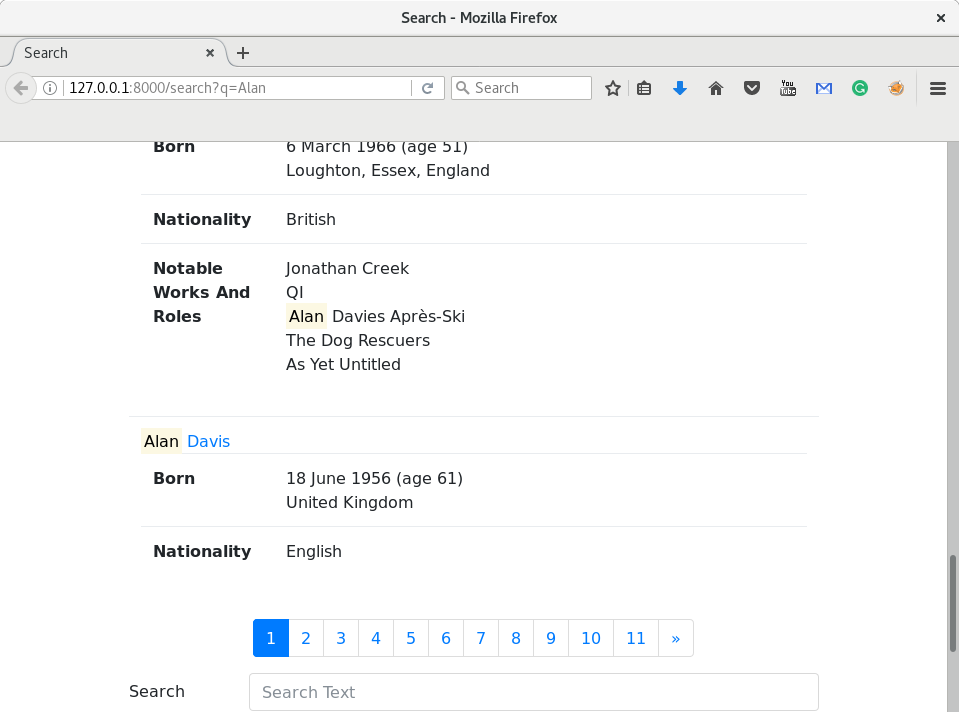
\includegraphics[width=\linewidth]{page.png}
	\end{subfigure}
	\hfill
	\begin{subfigure}{.49\textwidth}
		\centering
		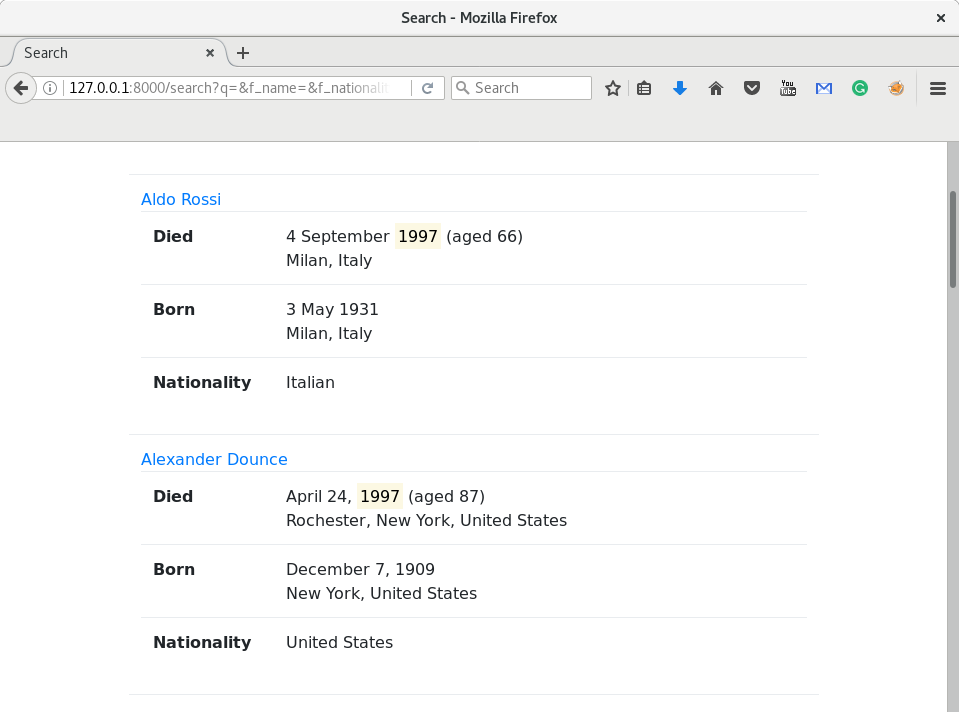
\includegraphics[width=\linewidth]{title-born.png}
	\end{subfigure}
	\caption{左侧为搜索结果过多时的分页显示效果,右侧为按照字段搜索Born中含1997的人物结果。}
\end{figure}


\begin{figure}[H]
	\centering
	\begin{subfigure}{.49\textwidth}
		\centering
		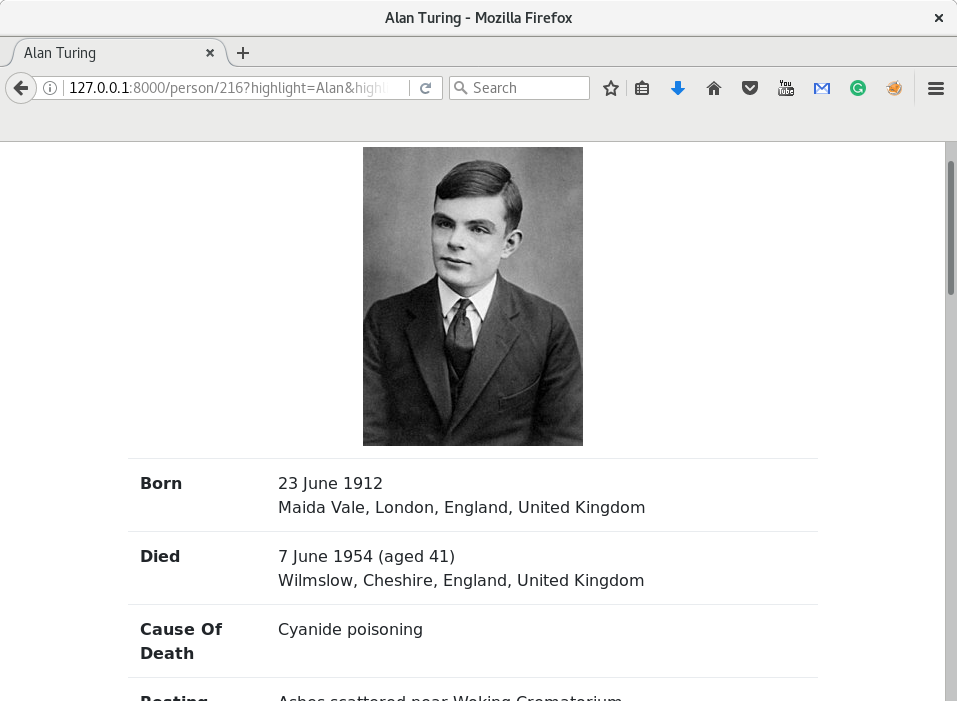
\includegraphics[width=\linewidth]{turing-1.png}
	\end{subfigure}
	\hfill
	\begin{subfigure}{.49\textwidth}
		\centering
		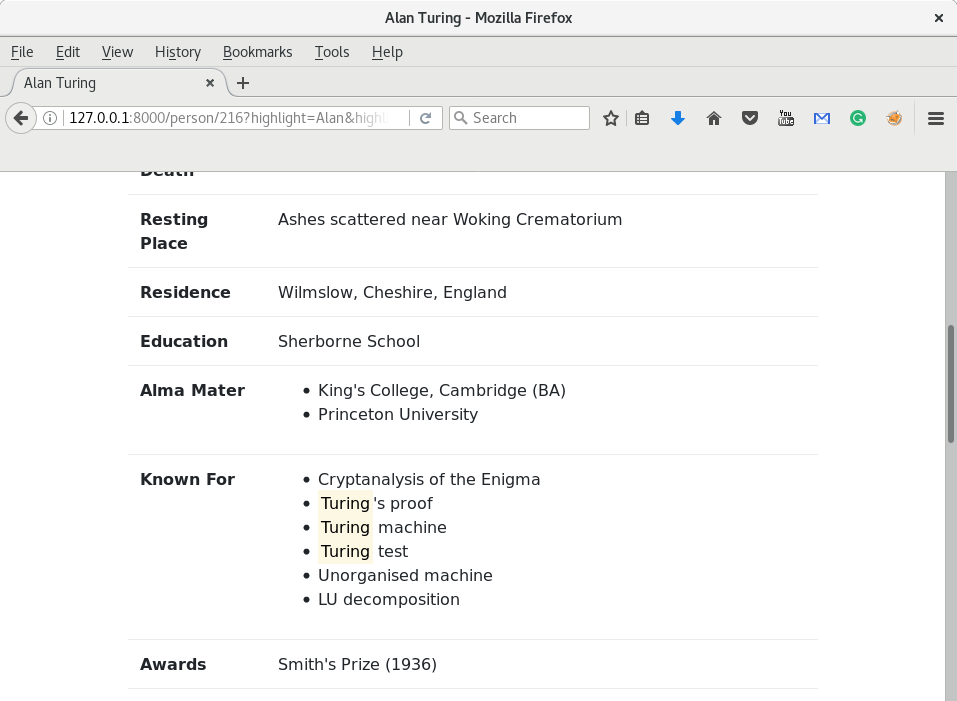
\includegraphics[width=\linewidth]{turing-2.png}
	\end{subfigure}
	\vspace{0.5cm}
	\begin{subfigure}{.49\textwidth}
		\centering
		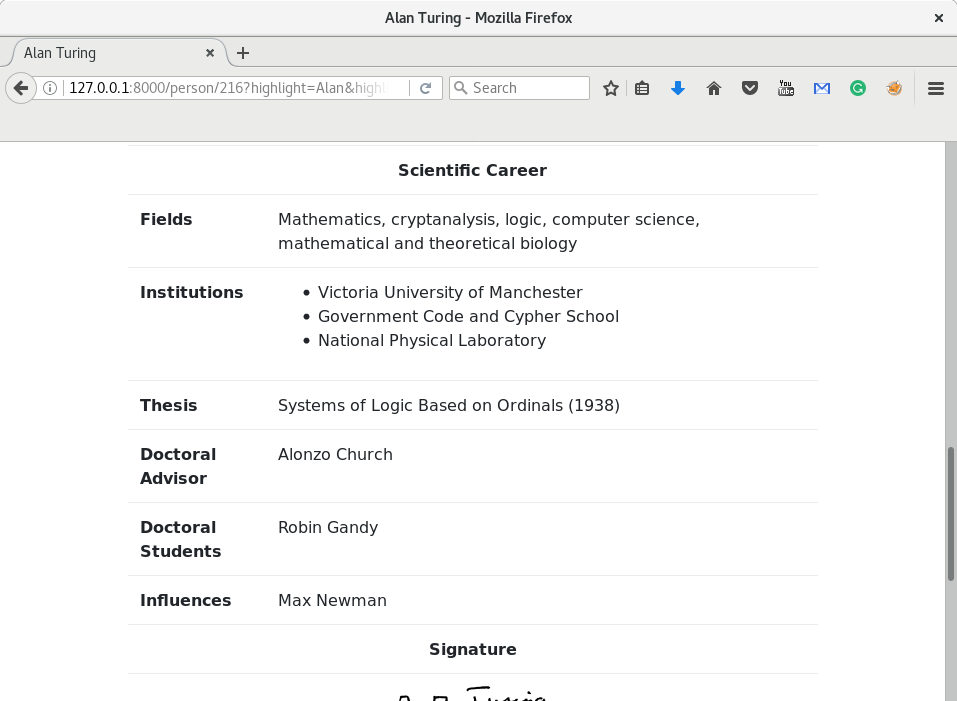
\includegraphics[width=\linewidth]{turing-3.png}
	\end{subfigure}
	\hfill
	\begin{subfigure}{.49\textwidth}
		\centering
		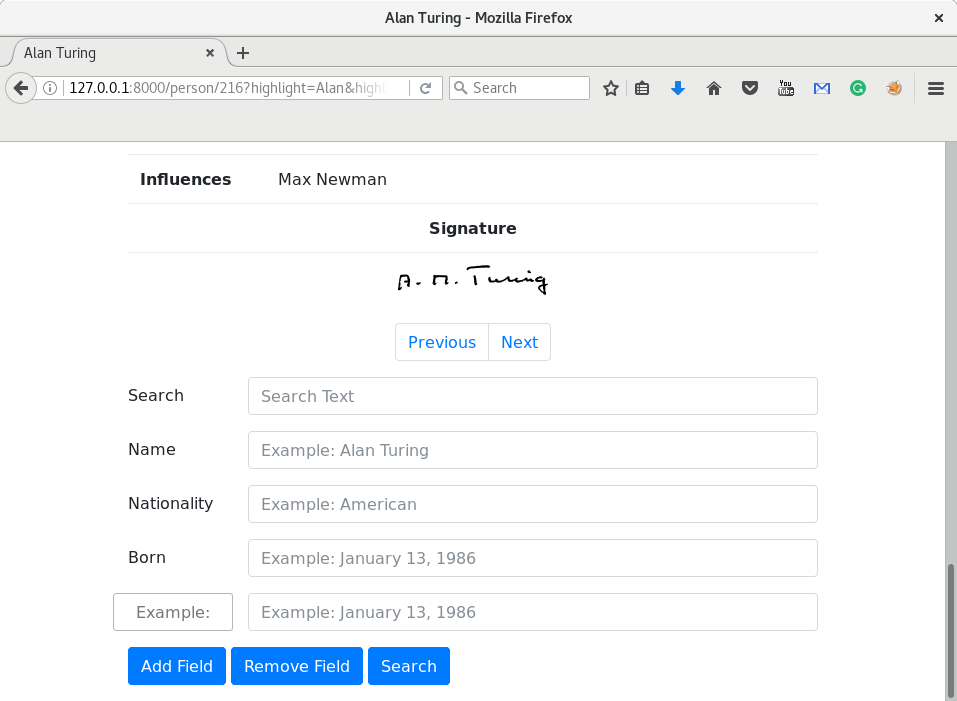
\includegraphics[width=\linewidth]{turing-4.png}
	\end{subfigure}
	\caption{Alan Turing信息的展现。}
\end{figure}

\section{部分实现细节}
爬虫部分利用BeautifulSoup来处理获取的页面,提取Infobox中的信息。

具体来说,人物超链接的爬取是通过寻找ID为{\it mw-content-text}的元素下所有{\it li}标签的第一个超链接来实现的。在爬取完毕后检查是否存在infobox,如果存在则开始提取信息。由于其中信息具有一定规律(例如大部分信息是以标题、内容的形式来组织的),只需要用BeautifulSoup提取相应的{\it <th></th>}以及{\it <td></td>}部分即可。

前端界面利用Bootstrap来优化显示效果。

关于数据的存储,在提取出信息后利用JSON来保存在sqlite数据库中,并且额外提取出一个关键字字符串用于搜索。对于每个人物都会分配一个唯一的ID以方便索引。

分页功能利用了Django自带的Paginator类。查询关键词的高亮以及自定义字段搜索框的增加与删除使用Javascript在前端完成。
\end{document}
